\chapter{vFIR Warszawa Airspace}%
\label{ch:airspace}
\section{Airspace Structure}%
\label{sect:airspace:structure}

\subsubsection{Controlled Airspace}
\begin{enumerate}[label={\alph*)}]
    \item CTA from FL95 to FL660 --- class ``C'' airspace,
    \item TMA, CTR --- below FL95 --- class ``C'' or ``D'' --- see ENR 2.1.1 or AD 2,
    \item MTMA, MCTR --- class ``D'' --- see ENR 2.1.1 or AD2,
    \item airspaces delegated to other FIRs --- see ENR 2.1.2
\end{enumerate}

\subsubsection{Uncontrolled Airspace}
Class ``G'' --- includes airspace from GND to FL95 outside of controlled airspace.

\subsubsection{Military Airspace}

Currently, only MCTR Dęblin, MCTR Krzesiny and MTMA Dęblin are simulated on the VATSIM network.

In the absence of vATC responsible for given military airspace, these airspaces are relegated to class G airspace.

The remaining military spaces are not currently simulated and have been relegated to Class G spaces.

\subsubsection{Reduced Vertical Separation Minimum (RVSM) in vFIR Warszawa}
vFIR Warszawa between FL290 and FL410 inclusive is an RVSM airspace.

In this airspace, the minimum vertical separation is:
\begin{description}
    \item[1000 ft] between aircraft authorized for RVSM operations.
    \item[2000 ft] between:
    \begin{itemize}
        \item aircraft authorized for RVSM operations and aircraft without such authorization,
        \item aircraft not authorized for RVSM operations,
        \item formation of aircraft and other aircraft.
    \end{itemize} 
\end{description}

\clearpage%
\section{Services Provided by ATC}%
\label{sect:airspace:services}

Within vFIR Warszawa the following Air Traffic Services are provided:
\paragraph{Air Traffic Control service}
\begin{description}
    \item[Aerodrome Control Service] --- for traffic in the Movement Area of an aerodrome and in the CTR,
    \item[Approach Control Service] --- for departing and arriving controlled flights,
    \item[Area Control Service] --- for controlled flights in CTAs. 
\end{description}

\begin{tcolorbox}[
    colback=orange!10!white,
    colframe=orange,
    title=\LARGE\textbf{Warning},
    before title={\faExclamationTriangle~}
]
    \textbf{Section under construction}
\end{tcolorbox}

\section{IFR flights}%
\begin{tcolorbox}[
    colback=orange!10!white,
    colframe=orange,
    title=\LARGE\textbf{Warning},
    before title={\faExclamationTriangle~}
]
    \textbf{Section under construction}
\end{tcolorbox}
\section{VFR flights}%
\begin{tcolorbox}[
    colback=orange!10!white,
    colframe=orange,
    title=\LARGE\textbf{Warning},
    before title={\faExclamationTriangle~}
]
    \textbf{Section under construction}
\end{tcolorbox}

\section{Squawk code assignment rules}%
\label{sect:airspace:squawks}

Virtual ATC of FIR Warszawa is provided with a pool of transponder codes ranging from 4500 to 4577. This gives a total of 64 different codes.

\begin{table}[htb]
    \centering
    \rowcolors{2}{vpink}{white}
    \begin{tabular}{|l|l|l|}
        \rowcolor{vred}
        \color{white}\textbf Sector & \color{white}\textbf Pool & \color{white}\textbf Codes\\\hline
        \textbf{ACC} \textit{(EPWW\_CTR)} & 4500 --- 4577 & 64\\\hline
        \textbf{Procedural TMAs} & 4500 --- 4517 & 16 \\\hline
        \textbf{TMA Poznań} & 4520 --- 4527 & 8\\\hline
        \textbf{TMA Gdańsk} & 4530 --- 4537 & 8\\\hline
        \textbf{TMA Kraków} & 4540 --- 4547 & 8\\\hline
        \textbf{TMA Warszawa} & 4550 --- 4577 & 24\\\hline
        \textit{\textbf{Reserve pool}} & 4000 --- 4077 & 64\\\hline
    \end{tabular}
    \caption{Squawk codes pool assignment}
    \label{tbl:squawk}
\end{table}

Transponder codes assigned in this way naturally run out when the most frequently occupied ATC positions are occupied and a standard traffic situation occurs. They should be awarded starting from the lowest number available.

When the controller is logged in at the ACC station, he is responsible for the final decisions regarding the allocation of transponder codes.

If the controller occupies a position in a sector other than those specified, he is obliged to consult the range or squawk codes for specific aircraft with the ACC controller, if logged in, if not, the controller should assign codes starting from the lowest available code from the basic range.

The presented code ranges are implemented in the official published sector and it is recommended to use automatically assigned codes during everyday work.

The controller occupying the procedural approach tower position in the appropriate TMA should assign the appropriate transponder code for departing aircraft only.

In case of heavy traffic, when the code pool is exhausted, a reserve range of 4000 --- 4077 is available.

VFR:\@ The default code for VFR flights is 7000. An aircraft flying with this code may be identified by radar by the controller in controlled airspace and provided with FIS/AFIS in Class G airspace using radar imagery, but only if the controller has a reasonable certainty regarding SP identification (no other traffic with the same transponder code within 20 NM). If there is no such certainty, the controller may assign a transponder code from the standard pool 4500 --- 4577.

The individually assigned unique transponder code should not be changed regardless of the aircraft's future route.

\subsection{Mode S transponder}

All aircraft flying in the area covered mode S identification (figure \ref{fig:modeS}) departing from an airport located in FIR Warszawa should receive squawk code 1000, and at the moment of obtaining radar contact, be identified as an aircraft communicating in mode S. If the aircraft flies outside the indicated space, a transponder discrete code in mode C should be assigned and identification should be made after take-off in accordance with applicable surveillance standards.

When accepting an aircraft currently in the air, identification in S mode occurs automatically. The discrete transponder code set by the pilot should be one of the following: 0000, 1000 (recommended, used in FIR Warszawa), 1200, 2000, 2200. If a different, discrete transponder code was assigned to the flight plan, identification should be made in mode C. If the aircraft shows a difference between the discrete code assigned in the flight plan and the one set on the transponder, identification cannot take place. Other conventional means of identification (described in ICAO Doc 4444, Chapter 8, points 8.6.2 and 8.6.3) are still available to the air traffic controller.

List of FIRs involving allocation of code '1000':

\-\hspace{1cm}EPWW, ED** (EDWW, EDMM, EDUU, EDGG), LKAA, LZBB, LROP, LHAA, EBBU, LOVV, LI**, LF** (LFFF + LFEE + LFMM + LFRR + LFBB)

List of aircraft equipment codes assigning the code "1000":

\-\hspace{1cm}H, I, L, E, G, W, P, S, LB1

\begin{figure}[htb]
    \centering
    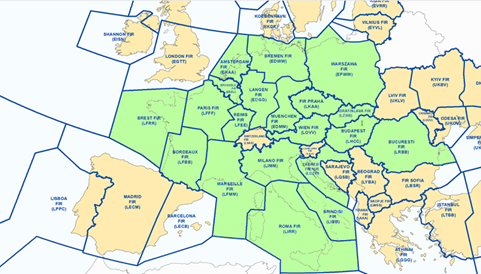
\includegraphics{modeS_FIRs.png}
    \caption{Mode S identification area map}
    \label{fig:modeS}
\end{figure}

In vFIR Warszawa, the \href{https://github.com/kusterjs/CCAMS}{CCAMS plugin} is used to assign transponder codes, which is an extension of the ModeS plugin.